\section{What the first responses count}
\label{sec:texts}

\subsection{Unpayable debts: the bound, to the dollar}
In 56 episodes the debt exceeds $U_*$. Eight of those menus offer bankruptcy alone. In the other 48 the agent could have financed or declared, and its first response usually says what its assets can raise. In 43 of the 48, the response contains the exact full bound, the exact proceeds $U_*-C$ or the exact gap $D-U_*$. Thirty of these figures are in authored notes and thirteen in provider fields. Grok's note in G15 is typical:
\QB{g15-max}
All four systems do this: Sol in 8 of 10 cases, Gemini in 11 of 11, Opus in 11 of 13 and Grok in 13 of 14. Two of the remaining five responses itemize every resource without a total. Three state the listed-only total (\S\ref{sec:false}).

\subsection{Payable debts that need released collateral}
Sixteen payable debts satisfy $U_0<D\le U_*$. Cash, every building and every listed mortgage together fall short, and the debt can be paid only with mortgages that a building sale releases. Agents paid fourteen. Figure~\ref{fig:sixteen} shows the sums and Appendix~\ref{app:texts} prints both text channels of all sixteen first responses in full.

\begin{figure*}[t]\centering
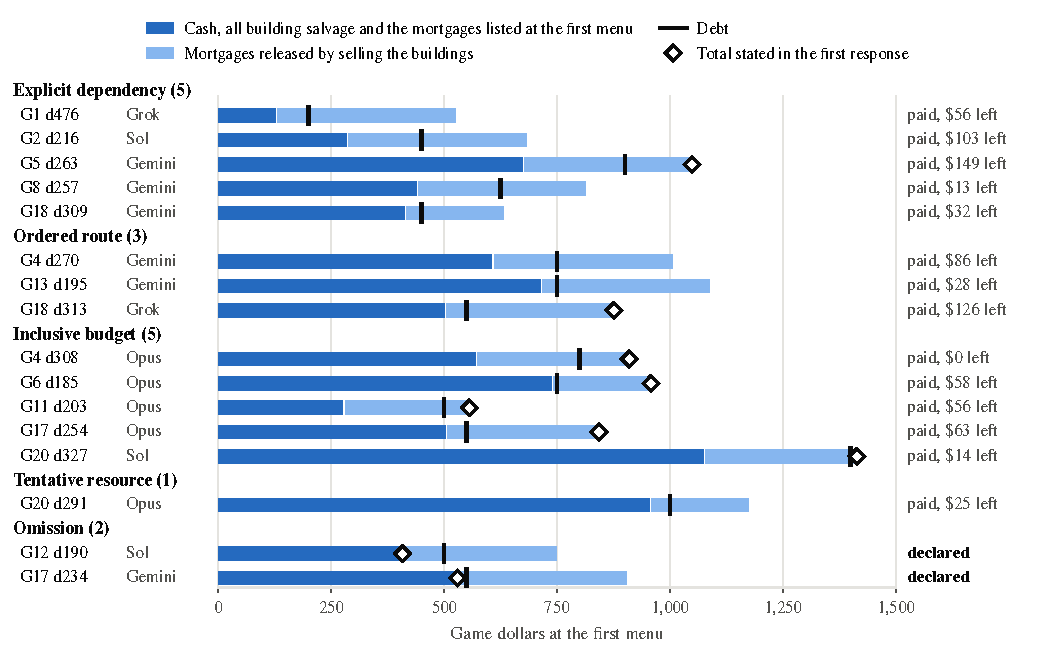
\includegraphics[width=.97\textwidth]{fig_sixteen.pdf}
\caption{The sixteen payable debts that required released collateral, grouped by how the first response treats that collateral. Every debt lies beyond the dark bar and within the pale one. A diamond marks a total stated in the response when it equals the listed-only total or the full bound (or the equivalent proceeds or remainder). Bars are resource sums, not liquidation plans.}\label{fig:sixteen}
\end{figure*}

The responses differ in how much they say about the dependency, and we sort them into five tiers (Table~\ref{tab:tiers}). Five state it. Grok writes \Q{g1-rule} Gemini writes that selling the houses \Q{g18-rule}. Three give an ordered route in which a sale precedes a named mortgage in the same group. Five give a budget that includes the locked deeds without saying what unlocks them. One raises the released mortgages as a question. Two leave them out.

\begin{table}[t]\centering\footnotesize
\begin{tabularx}{\linewidth}{@{}L{.25\linewidth}rY@{}}\toprule
Tier & $n$ & First responses\\\midrule
Explicit dependency & 5 & Grok G1; Sol G2; Gemini G5, G8, G18 d309\\
Ordered route & 3 & Gemini G4 d270, G13; Grok G18 d313\\
Inclusive budget & 5 & Opus G4 d308, G6, G11, G17 d254; Sol G20 d327\\
Tentative resource & 1 & Opus G20 d291\\
Omission & 2 & Sol G12 d190; Gemini G17 d234\\\bottomrule
\end{tabularx}
\caption{How sixteen first responses treat collateral that a sale must release. Tiers are one LLM author's reading of both channels, with evidence spans in Appendix~\ref{app:coding}.}\label{tab:tiers}
\end{table}

The tiers are not equally strong evidence. A statement or an ordered route shows that the response puts the sale first. An agent that summed every deed it owned would also write an inclusive budget. Four of the five inclusive budgets are Opus provider fields, the only channel Opus had, so tier and channel are confounded there.

The arithmetic is mostly right. In the authored notes and Opus's provider fields, every stated mortgage and resale value is correct except one: Sol gives the three yellow mortgages as \$430, and they total \$400. Seven successful responses contain a figure equal to the full bound, its proceeds or its remainder. Three state the cash that will remain, \$149, \$56 and \$14, and the route then leaves exactly that. Gemini's provider field in G5 shows an inventory being corrected inside one response:
\QB{g5-revise}

Errors and payment coexist. Sol's \$430 did not stop it paying. Opus in G20 d291 compares \$680 of proceeds with the whole \$1,000 debt and leaves out the \$275 it holds, so it calls itself \$725 short when the true gap is \$45. It then asks whether the pink deeds could be mortgaged once cleared, sells, and pays. In two of Gemini's successful responses the provider field ends before the released collateral appears, while the note in the same response states it. A provider field that stops early is therefore not evidence that the agent left a resource out.

\subsection{Two false budgets}
\label{sec:false}
Both failures among the sixteen are declarations at the first menu, and both follow a stated maximum:
\QB{g12-false-note}
\QB{g17-false-note}
Each sum is correct for what it counts, and each equals $U_0$ exactly. Sol leaves out \$340 of red mortgages and Gemini \$375 of dark-blue mortgages, the deeds their buildings stand on. The stored audit paid both debts from the same states with \$38 and \$180 to spare. Sol's provider field repeats the sum and continues \Q{g12-false-provider} Gemini's stops at \Q{g17-false-provider}

The same systems count the same kind of resource elsewhere. Sol pays two of its three debts in this group and Gemini five of six, one of them in G5 with the same two dark-blue deeds. The listed-only total is not confined to these two responses. Counting the sixteen payable debts and the 21 unpayable ones where buildings lock some deeds, 37 first responses face collateral that the menu does not list. Thirty-two count it or raise it. Five stop at the listed-only total: Sol twice, and Gemini, Opus and Grok once each. In three of the five the debt was unpayable either way, so the short count changed nothing. In the two payable cases it flipped the verdict.

The records do not say why these two inventories stopped where they did. Both agents carried earlier notes with the same reserve figures, \$130 and \$30. Those figures are also the true values of the listed mortgages, so the match cannot separate reuse of a note from a fresh count of the menu, and similar carried figures precede four payments in this group (Appendix~\ref{app:carried}). Counting what the menu lists, reusing an inventory written while the buildings were meant to stand, applying a known rule incompletely, and ordinary response variation all fit two cases. Sol's remark about property transfer shows that a declaration can also rest on more than the budget, and the prompt allows a player to stop when it ``cannot or should not'' raise the cash. The two budgets are false statements about what could be raised. Whether they were the whole reason for stopping is not identified.

\subsection{Choosing what to give up}
The engine stops asking once cash covers the debt, so the order of an agent's actions decides what it gives up. Sixty-two payments had enough cash and listed mortgages. The player held buildings in thirty of them, and in 28 it paid by mortgages alone and kept every building. In the 52 payments that needed sales but no released mortgage, 46 kept some buildings. Across all 128 payments, 122 left a deed unmortgaged, and in 119 the cash left over was smaller than the smallest house or mortgage given up, so no single unit in the route was surplus. We did not search for cheaper routes.

\incident{1}{A plan that names what to keep (G13).} Gemini owes \$750 with \$168. Its note sets the route:
\QB{g13-select}
The engine records one house sold, then Pacific, Electric Company, Indiana and Park Place mortgaged, for \$28 left. Boardwalk and Kentucky stay unmortgaged as planned. The bound here was \$1,088, so Gemini had \$338 of slack and chose which assets to spend. Its provider field gives the reason: \Q{g13-select-why}

\incident{2}{An exact budget on both sides of a debt (G20).} The note in Gemini's hotel build reads \Q{g20-creditor} Here p3 is Sol, and the two components are each \$25 off and cancel. Sol's note at the debt states the same \$1,414 and a \$14 remainder. At its tenth call the note reads \Q{g20-last} The debt sat \$14 below the bound, so full liquidation was the only end state that paid. The case shows two agents valuing nineteen assets to the dollar, not a choice among routes.
